\documentclass[../main.tex]{subfiles}


\begin{document}

\chapter{Terningen: Data og repræsentation}
\lhead{Data}
\section{Matematikken bag tilstandsrummet}\label{sec:grouptheory}
For at motivere sværhedsgraden af problemet, vil aspekter ved Rubiks terning blive beskrevet ud fra et gruppeteoretisk perspektiv. Dette afsnit bygger hovedsageligt på \cite{GroupTheory}, men er tilpasset vores egen repræsentation og implementation af Rubiks terning. 
\subsection*{Permutationer}

Rubiks terning har seks sider og 26 cubies i alt; seks midtercubies med én udadvendt overflade, 12 kantcubies med to flader og otte hjørnecubies med tre flader. Hver side kan roteres $\frac{\pi}{2}$ radianer med eller mod urets retning. Fastholdes orientationen af Rubiks terning, vil positionen af alle centercubies også holdes fast, uafhængigt af hvordan siderne roteres. Således vil man kunne navngive hver side ud fra dens orientation, og vi har nu front F, bag B, op O, ned N, højre H og venstre V. De otte omkringliggende cubies på hver side nummereres som vist på Figur \ref{RubiksImplementation}. Bemærk, at lige numre svarer til en kantcubie og ulige numre svarer til en hjørnecubie.

\begin{figure}[H]
	\centering 
	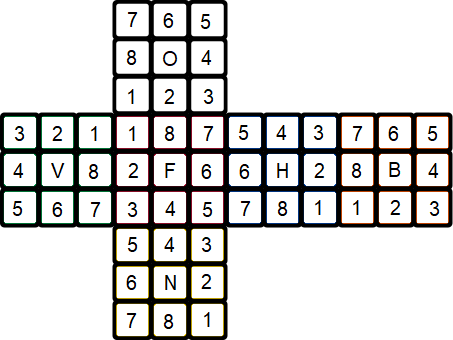
\includegraphics[width=.5\linewidth]{rubiks_implementation}
	\caption{Repræsentation af Rubiks terning.}
	\label{RubiksImplementation}
\end{figure}

Ud fra kvart-drejnings-semantikken kan man foretage 12 forskellige handlinger på Rubiks terning (13 hvis man medtager handlingen ikke at foretage nogen handling); hver side kan roteres én gang enten med eller mod uret. Notationsmæssigt betyder rotationen F, at frontsiden set fra observatørens perpektiv roteres $\frac{\pi}{2}$ radianer i urets retning. 2F svarer til en rotation af fronten på $\pi$ radianer, og 3F = F' svarer til én rotation mod urets retning. 

En rotation kan ses som en permutation af Rubiks terning. En permutation $f:A\rightarrow A$ en afbildning af mængden A på sig selv. En rotation kan skrives som en permutation bestående af fem disjunkte 4-cykler. Ud fra navngivningen i Figur \ref{RubiksImplementation} vil rotationen F kunne skrives som

$$F:(\begin{matrix}f_1 & f_7 & f_5 & f_3\end{matrix})
(\begin{matrix}f_2 & f_8 & f_6 & f_4\end{matrix})
(\begin{matrix}v_1 & o_3 & h_7 & n_5\end{matrix})
(\begin{matrix}o_2 & h_6 & n_4 & v_8\end{matrix})
(\begin{matrix}o_1 & h_5 & n_3 & v_7\end{matrix})$$

Ligeledes kan resten af permutationerne F', B, B', O, O', N, N', H, H', V og V' hver skrives som en kombination af fem disjunkte 4-cykler. Ikke at foretage en rotation navngives I.


\subsection*{Rubiks terning som en gruppe}
Mængden $\{F, F', B, B', O, O', N, N', H, H', V, V', I\}$ er en permutationsgruppe $(\mathbb{G}, *)$ med gruppeoperatoren $*$ defineret som følger; $X*Y$ er udførelsen af handling X efterfulgt af handling Y. $\mathbb{G}$ opfylder forudsætningerne for en permutationsgruppe: 
\begin{itemize}
	%\item $\mathbb{G}$ er lukket, så hvis $X*Y=Z$ er Z også et element i $\mathbb{G}$. 
	\item $\mathbb{G}$ er associativ, eftersom $(X*Y)*Z=X*(Y*Z)$; at foretage handling X og Y efterfulgt af Z er det samme som at foretage handling X efterfulgt af Y og Z. 
	\item $\mathbb{G}$ har et identitetselement I (ikke at foretage en handling), eftersom $I*X = X = X*I$. 
	\item Hvis X er et element i $\mathbb{G}$ har X en invers $X^{-1}$ således at $X*X^{-1}=I$. Dette er opfyldt, eftersom  $X^{-1}=X'$.  
\end{itemize} 

Med denne viden om $\mathbb{G}$ og Rubiks terning kan vi nu beregne antallet af permutationer (ordenen af $\mathbb{G}$). Først beregnes alle permutationer, både lovlige og ulovlige. Dette svarer til alle kombinationer, hvor man fysisk tager en cubie og placerer den, som man vil. Der er otte pladser til hjørnecubies, som hver har tre måder at blive orienteret på. Der er 12 pladser til kantcubies, som hver har to måder at blive orienteret på. Eftersom midtercubies er fikserede, fås 

$$8!\cdot3^8\cdot12!\cdot2^{12}=519.024.039.293.878.272.000=5,2\cdot10^{20}$$

permutationer. Der skal dog tages højde for ulovlige permutationer. Af disse er kun halvdelen af kantcubies placeret lovligt og en tredjedel af hjørnecubies placeret lovligt. Endvidere er der i halvdelen af permutationerne blevet udskiftet et ulige antal cubies, hvilket er umuligt. Derfor her vi

$$\frac{8!\cdot3^8\cdot12!\cdot2^{12}}{2\cdot3\cdot2}=43.252.003.274.489.856.000=4,3\cdot10^{19}$$

lovlige permutationer. Dette er ligeledes størrelsen på tilstandsrummet for problemet.

\subsection*{Guds tal}
Inde for Rubiks terning betegnes det mindste antal træk der skal til for at løse en terning som Guds tal. Betegnelsen \emph{Guds tal} kommer af, at man er nødt til at være et altvidende væsen for at kunne løse enhver af de $4,3\cdot10^{19}$ permutationer på dette antal træk eller færre. Dette tal er 26 eller færre i kvart-drejnings-semantik og blev fundet tilbage i 2014 ved essensielt at bevise, at alle permutationer af Rubiks terning kan løses på 26 eller færre træk \cite{10.4169/college.math.j.45.4.242}. Fremgangsmåden var at dele alle permutationer op i $2,2\cdot10^9$ sæt med $2,0\cdot10^{10}$ permutationer i hver, som derefter vha. symmetri og sætdækning kunne reduceres til i alt $5,6\cdot10^7$ sæt, der skulle løses. For hvert sæt fandt de (ved brug af særligt stor computerkraft) løsninger på længden 26 træk eller mindre, og Guds tal er derfor nu 26. 



\section{Repræsentation af terninger}\label{sec:repr}
Der findes en lang række måder at repræsentere tilstanden af en terning på.
For at opnå de bedste resultater, skal den valgte repræsentation
\begin{itemize}
	\item undgå overflødighed
	\item bruge lidt hukommelse
	\item kunne foretage rotationer hurtigt
	\item fungere godt med neurale netværk
\end{itemize}
Den mest oplagte måde at repræsentere terningen på er en $ 6\times 9 $-tensor, hvor hver indgang er et tal svarende til en farve.
Det er dog ikke nødvendigt at modellere det midterste kvadrat, så længe terningens orientering er fastlagt, hvilket reducerer repræsentationen til $ 6\times 8 $.
Denne repræsentation bruger kun $ 6\cdot 8\cdot 4=192 $ bytes, når tallene gemmes som 32 bit floating points.
Det er også muligt at foretage rotationer hurtigt, men det er muligt at repræsentere en lang række tilstande, der ikke ligger i tilstandsrummet -- fx at alle kvadrater på alle sider har samme farve.
Med seks farver består det repræsenterbare tilstandsrum af $ 6^{6\cdot 8}\approx 2,25\ctp{37} $ tilstande, langt større end de $ 4,3\ctp{19} $ lovlige tilstande.
Repræsentationen er heller ikke velfungerende med neurale netværk, hvor one-hot encoding er at foretrække.
Ved at tilføje en ekstra akse til tensoren er one-hot muligt, men det kræver $ 6\cdot 8\cdot 6\cdot 4=1152 $ bytes og løser stadig ikke overflødighedsproblemet.\\
\\
En anden, mindre intuitiv repræsentation er en $ 20\times 24 $-tensor.
Forestiller man sig Rubiks terning som bestående af 26 mindre kuber (foruden den i midten af terningen) og fjerner de seks midterkuber, fås 20 kuber, der skal repræsenteres.
Disse inkluderer 8 hjørnekuber og 12 sidekuber.
Hjørnekuberne kan sidde 8 steder og have tre forskellige orienteringer, hvilket giver 24 mulige tilstande.
Tilsvarende kan sidekuberne sidde 12 steder med to orienteringer, hvorfor de også har 24 mulige tilstande.
Kvadraterne på hver kube har en unik farvekombination,\footnote{Det er muligt at overbevise sig selv om det ved at forestille sig den løste terning.} og det er derfor muligt at repræsentere hver kube ved blot ét af dens kvadrater.
Repræsentationen er visualiseret på figur \ref{fig:kuberepr} og følger direkte repræsentationen i \cite{HumansBeGone}, hvorfra illustrationen også er taget.
\begin{figure}
	\centering
	\includegraphics[width=\textwidth]{repr}
	\caption{Repræsentation af Rubiks terning. Der holdes styr på de hvide kvadrater på (c) og (d). \cite{HumansBeGone}}\label{fig:kuberepr}
\end{figure}
Denne repræsentation kan repræsentere $ 24^{20}\approx 4,02\ctp{27} $ tilstande -- et stykke over tilstandsrummets størrelse, men stadig langt bedre end det omtalte alternativ.
Til gengæld kræver det $ 20\times 24\times 4=1920 $ bytes at gemme en tilstand, men rotationer kan foretages hurtigt.
Endeligt er tilstande one-hot encodede, hvilket gør det anvendeligt til neurale netværk.
Samlet set vurderes denne repræsentation til bedre at opfylde kravene, hvorfor den anvendes.


\end{document}






















